\documentclass[10pt,a4paper]{article}
\usepackage[margin=2.2cm]{geometry}
\usepackage[T1]{fontenc}
\usepackage{lmodern}
\usepackage{microtype}
\usepackage{graphicx}
\usepackage{booktabs}
\usepackage{amsmath}
\usepackage{siunitx}
\usepackage{xcolor}
\usepackage[hidelinks]{hyperref}
\usepackage{caption}
\captionsetup{font=small,labelfont=bf}

\title{\textbf{Duckophila: a whole-brain \emph{Drosophila} connectome model in closed loop with a bipedal robot}\\[0.4em]
\large Technical report and preprint draft}
\author{Helge Winkler\\\small\texttt{hw@alphasix.de}\\\small\url{https://github.com/first-it-consulting/duckophila}}
\date{November 2026}

\begin{document}
\maketitle

\begin{abstract}
We connect the complete connectome-derived leaky integrate-and-fire model of the adult \emph{Drosophila
melanogaster} brain (FlyWire, 138{,}639 neurons, 54.5 million synapses; Shiu et al.\ 2024) to a small
bipedal robot, the open-source microduck of Pollen Robotics (Hugging Face), running its production control software against a MuJoCo
simulation of its body. The robot's time-of-flight depth sensor is translated into input to the fly's
looming-sensitive visual projection neurons (LPLC2, LC4); its camera, through dense optic flow, into input
to the fly's elementary motion detectors (T4/T5), each placed at its own visual column using FlyWire's
column map. Motor commands are read out from identified descending neurons. Without any tuning of the
connectome, the model (i) fires its giant fibre (DNp01) to objects approaching the robot's face (20 of
20 throws in closed loop), and (ii) produces a syndirectional optomotor response in DNp15/DNHS1 that turns
the robot's head---and, through a coupling rule of ours, its walking body---with a rotating striped drum,
at a closed-loop gain of 0.23 [0.21, 0.27], and (iii) turns the walking robot toward a small target
through LC10a, the anterior optic tubercle and DNa02, keeping up with a target led \SI{90}{\degree} each
way in 4 of 8 runs (heading gain 1.00). All three require the wiring: a degree-preserving rewired
connectome with the same neurons and weights produces none (0 of 20; gain 0.00; 0 of 8). Further controls show
that DNp15 is the strongest rotation-following neuron of 383 paired descending neuron types, while the
escape response is only partly specific to the looming detectors and only weakly lateralised, and that
the target pathway steers only for targets below the eye's equator, and more weakly to the right.
The model's mushroom body, in contrast, has no input-specific code: any input that reaches it recruits
the same two-thirds of its Kenyon cells, through a runaway that starts in the antennal lobe. With
cue codes, a dopamine plasticity rule and a valence readout supplied by us, the robot learns to
approach whichever of two targets it was petted for (5 of 6 runs; the other, 0 of 6). With a
motion-based encoder for a real room the same pathway turns the robot after a person's feet (heading
gain 0.67 against 0.02 rewired) and, in 3 of 8 runs, walks after one (0 of 8 rewired), though only with
a readout, a correction and control rules of ours, listed. The brain can
also drive the robot from a laptop over WebRTC, with every camera frame dated on the robot's clock. To run the model in closed loop we reimplemented it as a stepped
simulator that reproduces the reference Brian2 implementation spike for spike and runs faster than real
time on one CPU core, using an exact closed-form bound that lets neurons unable to fire before their next
input remain unsimulated. We report what the connectome contributes, what our hand-written sensory and
motor interfaces contribute, and several failure modes found on the way: a dropped-input rule of the
reference model, scrambled retinotopy destroying LPLC2 selectivity, the robot's own gait dominating its
optic flow, and a field of view too narrow for the canonical steering neuron DNa02. Code, experiments and
a recorded demonstration are open source.
\end{abstract}

\section{Introduction}

Complete synaptic wiring diagrams of an adult insect brain now exist. FlyWire reconstructed the whole
brain of a female \emph{Drosophila} \cite{dorkenwald2024}, annotated every neuron with a cell type
\cite{schlegel2024}, and mapped the visual system to its retinotopic columns \cite{matsliah2024}. Shiu et
al.\ \cite{shiu2024} showed that a leaky integrate-and-fire (LIF) network built directly from this
connectome---every synapse at one shared weight, its sign taken from the predicted neurotransmitter---
predicts sensorimotor pathways that were then confirmed experimentally, for example from sugar-sensing
gustatory neurons to the proboscis motor neuron MN9.

That model has so far been driven by prescribed stimulation and read out offline. Here we ask a
different question: what does it do when its sensory neurons are driven by a robot's sensors, its
descending neurons move that robot, and the consequences of those movements come back through the
sensors---in closed loop, in real time? The robot is the microduck, a 15-servo bipedal robot from Pollen
Robotics with an 8$\times$8 time-of-flight (ToF) depth sensor and a head camera, controlled by
reinforcement-learned locomotion policies. We do not replace the robot's locomotion: the fly brain sits
above it, as a behaviour source, the way descending neurons sit above the fly's ventral nerve cord.

Our contribution is an engineering study with three parts: (1) a stepped, exact and faster-than-real-time
reimplementation of the Shiu et al.\ model; (2) sensory interfaces that respect the fly's own anatomy---in
particular a retinotopic placement of every T4/T5 neuron whose orientation is derived from the connectome
itself; and (3) closed-loop experiments in a simulated twin of the robot that runs the robot's production
daemons. Throughout, we separate what the connectome does from what our interfaces do, because that
boundary is what any claim about ``a fly brain controlling a robot'' depends on (Table~\ref{tab:boundary}).

\begin{table}[t]
\centering\small
\caption{What is the connectome's and what is ours. The brain model is not trained, tuned or edited.}
\label{tab:boundary}
\begin{tabular}{p{0.45\linewidth}p{0.47\linewidth}}
\toprule
From the connectome (unchanged) & Hand-written interfaces (ours) \\
\midrule
Every neuron, synapse and sign; the LIF dynamics of \cite{shiu2024} & ToF $\rightarrow$ LPLC2/LC4 Poisson rates (inverse time-to-contact) \\
Which neurons respond to looming, which to rotation & Camera $\rightarrow$ optic flow $\rightarrow$ T4/T5 rates by preferred direction \\
That the giant fibre fires (and more reliably for LPLC2/LC4 input) & The shape of the startle (sound, gaze, crouch, step back) \\
The sign and size of the DNp15/DNa02 left--right difference & Gains, smoothing, clamps; the body following the head \\
Where each T4/T5 looks (FlyWire columns); front and up, from the wiring & Approach-speed gate; efference copies of the robot's own motion \\
That LC10a $\rightarrow$ AOTU019/025 $\rightarrow$ DNa02 turns toward a small target, only below the equator & Target detector; bearing $\rightarrow$ LC10a rates and their dose; walking while a target is seen \\
Which DN pairs carry a target's bearing; that two feet steer and whole legs do not & For a person: moving things as point targets at their lowest \SI{8}{\degree}; the room's homography; level elevation; a four-DN readout and its lean; distance keeping, heading memory, suppression, search, pursuit gate \\
Kenyon cells $\rightarrow$ MBONs $\rightarrow$ downstream; which DANs reach which MBON & Learning: cue codes, plasticity rule, valence by compartment, antennal lobe silenced, approach gate \\
\bottomrule
\end{tabular}
\end{table}

\section{Methods}

\subsection{Brain model and a stepped reimplementation}

We use the FlyWire 783 connectome as distributed with \cite{shiu2024} (138{,}639 neurons, 15{,}091{,}983
connected pairs, 54{,}492{,}922 synapses) and the model's equations and constants unchanged: membrane
time constant \SI{20}{ms}, synaptic time constant \SI{5}{ms}, rest and reset \SI{-52}{mV}, threshold
\SI{-45}{mV}, refractory period \SI{2.2}{ms}, synaptic delay \SI{1.8}{ms}, \SI{0.275}{mV} per synapse,
time step \SI{0.1}{ms}, and Poisson stimulation as a voltage kick of $250 \times \SI{0.275}{mV}$.

The reference implementation in Brian2 \cite{stimberg2019} rebuilds the network for every run, which is
appropriate for one-second optogenetic trials but not for a sensorimotor loop that needs tens of
milliseconds of brain time per sensor frame (a \SI{20}{ms} step cost \SIrange{0.2}{0.4}{s} of wall time;
a long run, 2.6$\times$ real time). Our stepped simulator (\texttt{flysim.py}, numba) holds the state
between calls and follows Brian2's schedule within each step: state update, threshold, synaptic
propagation and Poisson input, reset.

\paragraph{A semantic detail of the reference.} In the reference model $v$ and $g$ are declared
\texttt{(unless refractory)}. Brian2 implements this as a \emph{conditional write}: any write to these
variables, including synaptic input, is discarded while the neuron is refractory. Input arriving during
refractoriness is therefore lost, not accumulated. An implementation that banks it is plausible-looking
but wrong: every downstream neuron fired $\sim$20\% too fast in ours until this was matched. We found it by
replaying the reference's own input spike times into our simulator and comparing every downstream spike.

\paragraph{Exact sparsity.} Under strong visual drive $\sim$50{,}000 neurons sit just off rest, and
stepping them made the brain four times slower than real time; parallelising the per-step pass across
cores made it slower still (thread-region launch every \SI{0.1}{ms}). Between inputs the model is linear,
so the highest a neuron's voltage can still reach without further input has a closed form:
\begin{equation}
v_{\max} - v_0 \le \max(u,0) + P_g \max(g,0),\qquad P_g = \max_t \frac{\tau}{\tau - T}\left(e^{-t/\tau}-e^{-t/T}\right) \approx 0.157,
\end{equation}
with $u = v - v_0$, $T$ the membrane and $\tau$ the synaptic time constant. A non-refractory neuron whose
bound is below threshold cannot spike before its next input; it becomes \emph{dormant} and is not stepped.
Its next synaptic arrival or Poisson event wakes it, and its state is advanced analytically over the gap
(the per-step propagator raised to the gap, from a lookup table). Poisson input is drawn as geometric
inter-event gaps per frame rather than a Bernoulli trial per neuron per step, which is the same process.
The result remains spike-for-spike identical to Brian2 under replay (13{,}607 of 13{,}607 spikes) while
cost follows synaptic events instead of neurons $\times$ steps.

\subsection{Robot, simulator and interface}

The microduck's production daemons (\texttt{robotd}, \texttt{tofd}, \texttt{mediad}) run unmodified
against a MuJoCo \cite{todorov2012} model of its body, with only the servo bus, the ToF sensor and the
camera replaced by the simulator (\texttt{scripts/duck-sim}). Our bridge reads the robot's own interfaces:
ToF frames at \SI{15}{Hz} (\texttt{tof.stream}), camera frames at \SI{30}{Hz} (\texttt{media.frame}), and
the robot's state at \SI{50}{Hz} (\texttt{robot.state}: head forward kinematics, IMU orientation,
odometry, executed twist). It writes only intents the robot already accepts---\texttt{robot.move},
\texttt{robot.head}, \texttt{robot.look}, \texttt{robot.pose}, \texttt{robot.sound}. The brain advances by
exactly the time between ToF frames, with the latest camera-derived rates.

A stimulus prop (a sphere that can be thrown at the robot) and a rotating drum of 48 alternating black and
white panels (\SI{0.5}{m} radius, a \SI{15}{\degree} spatial period) are added to the simulator without
modifying it: a generated copy of the scene, and a Python start-up hook that moves the two mocap bodies.

\paragraph{The twin had to walk first.} The twin as shipped loaded an obsolete walking policy on a robot
model without joint backlash, and did not walk: \SI{4}{cm} in \SI{8}{s} at \SI{0.15}{m/s} commanded.
The current policy (velstand) was trained with backlash and stands still without it; with both corrected
the twin walks (\SI{0.06}{m/s} for \SI{0.15}{m/s} asked) and turns (\SI{50}{\degree/s} for
\SI{46}{\degree/s} asked on the spot). This fix has been submitted upstream. The residual shortfall in
forward speed, a dead band below $\sim$\SI{0.55}{rad/s} of yaw on the spot, and an occasional failure to
take a first slow step are properties of the twin that our controllers have to live with.

\paragraph{Off the robot.} On hardware the brain runs on a laptop and reaches the robot over the
WebRTC session the robot publishes: the camera as an H.264 track and the robot's JSON-RPC interface
over a data channel (\texttt{link.py}). WebRTC frames carry no capture time, so each is dated from
the RTCP sender reports and a pair of robot clock readings onto the robot's monotonic clock, the one
its state stream is stamped with; frame and state then pair without the network delay. Against the
simulated robot's media daemon, following, the startle and the head reflex (gain 0.24 [0.19, 0.28],
against 0.23 locally) work over this path.

\subsection{Startle: depth sensor to looming detectors}

The giant fibre (DNp01, one per side) receives its two largest excitatory inputs from LPLC2 and LC4
(10.6\% and 8.6\% of the left GF's annotated input synapses; 12.1\% and 8.4\% of the right's), consistent
with their established roles in looming detection \cite{vonreyn2017,ache2019,klapoetke2017}. For each ToF
zone we estimate inverse time-to-contact $\tau^{-1} = -\dot d/d$ from a line fit over four frames
(\SI{0.27}{s}); a zone drives the LPLC2 and LC4 neurons assigned to it (left four columns to the left optic
lobe, round-robin within a side, $\sim$3 LPLC2 and $\sim$1.5 LC4 per zone) at a saturating rate up to
\SI{150}{Hz}. Two filters are ours and labelled as such: zones whose return is the floor are excluded,
using the robot's own floor test with a \SI{3}{\degree} pose margin; and drive is gated on approach speed
above \SI{0.4}{m/s}, a duck choice that loosely parallels the giant fibre's preference for fast looming
\cite{vonreyn2017}. A giant-fibre spike triggers a startle assembled from existing intents, with a \SI{2}{s}
refractory period.

\subsection{Optomotor reflex: camera to motion detectors}

\paragraph{Retinotopy from the connectome.} Each eye has $\sim$750 T4 and $\sim$750 T5 neurons of each of
four preferred directions (a front-to-back, b back-to-front, c up, d down \cite{maisak2013}). FlyWire's
column map \cite{matsliah2024} assigns 11{,}822 of them to 796 hexagonal columns (395 left, 401 right)
with axial coordinates $(p,q)$. Nearest neighbours differ by $(p{+}1, q{+}1)$ or by one coordinate, which
gives physical coordinates $X = \sqrt3\,(q-p)/2$, $Y = (p+q)/2$ and a roughly round eye.

The map does not say which direction is anterior or dorsal. We derive both from the wiring
(Fig.~\ref{fig:eyes}). LPLC2's four dendritic arms each take the T4/T5 subtype whose preferred direction
points away from the cell's centre \cite{klapoetke2017}; averaging, over all LPLC2 of an eye, the position
of each subtype's inputs relative to the cell's input centroid places T4a/T5a at $\Delta X = -2.7$ and
$-2.9$ columns (left and right eye), T4b/T5b at $+2.1$ and $+1.9$, T4c/T5c at $\Delta Y = +1.7$ and $+1.9$,
and T4d/T5d at $-2.1$ and $-2.2$. Hence $+X$ is anterior and $+Y$ dorsal in both eyes. Independently, the
dorsal and ventral HS cells (HSN, HSS) take their T4/T5 input at higher and lower $Y$ respectively,
confirming the vertical axis, and the equatorial HSE sets elevation zero. With an interommatidial angle of
\SI{4.8}{\degree} and the frontmost column placed \SI{10}{\degree} across the midline, the eyes span
\SIrange{-10}{131}{\degree} in azimuth and \SIrange{-84}{66}{\degree} in elevation.

\paragraph{Flow to rates.} The camera sees \SI{45}{\degree}$\times$\SI{73}{\degree} straight ahead.
Only T4/T5 neurons whose direction falls in that view---1{,}424 of 11{,}822---receive input: dense
Farneb\"ack optic flow \cite{farneback2003} at quarter resolution, averaged over one column's extent at the
neuron's position, projected on its preferred direction, rectified and mapped to a saturating Poisson rate
($\le$\SI{60}{Hz}). Image left is the robot's left (verified with a placed object).

\paragraph{Efference copies.} Image motion the robot causes deliberately is predicted and subtracted
before it reaches the fly: the head's idle look-around, and walking. Walking turned out to be dominated not
by translation (floor flow $\sim$\SI{10}{\degree/s} at \SI{0.08}{m/s}) but by the gait's pitch and roll
(\SIrange{30}{80}{\degree/s}). We predict both per pixel from the robot's state---floor translation from
odometry on pixels whose ray meets the floor, rotation from the camera's world orientation between states
with the vertical component removed (yaw slip is the reflex's own signal)---and subtract the prediction
weighted by local image texture, since a flow estimator, like a T4 neuron, reports no motion on an edgeless
surface. The prediction matches a controlled head nod with $r = 0.98$; during walking it correlates with
the measured flow ($r = 0.90$) only when each frame is paired with the state at its own capture time.

\paragraph{Motor readout.} DNp15 (DNHS1 \cite{namiki2018}) left--right difference, smoothed
(\SI{0.15}{s}), integrates into head yaw. For the body we tested DNa02 \cite{rayshubskiy2020} directly
(\texttt{--steer dna02}) and a head-led coupling of ours (\texttt{--steer body}): the walking body
(\SI{0.1}{m/s}) turns at $k \cdot$ head yaw while the head counter-rotates by the trunk's measured yaw
rate, so gaze is held.

\subsection{Following: a camera target to the small-object pathway}

FlyWire's brain is female, so it lacks P1 and the courtship-pursuit circuit. It does contain the visual
object pathway that pursuit uses: LC10a, lobula columnar neurons tuned to small moving objects
\cite{ribeiro2018,hindmarshsten2021}, project to the anterior optic tubercle, whence AOTU019 (GABAergic,
mostly onto the contralateral DNa02) and AOTU025 (cholinergic) reach DNa02. We locate each LC10a's
receptive field as the synapse-weighted mean viewing direction of its inputs that lie on the column map
(Tm20, Tm4 and others), on its own eye: 232 of 234 LC10a receive such input. The target---in simulation a
small self-lit sphere, the only saturated object in the grey camera image, found as the largest bright blob
after a morphological opening---gives a bearing and elevation through the pinhole model, and drives each
LC10a at $r_{\max}\exp(-d^2/2\sigma^2)$, $d$ the angle between target and receptive field
($r_{\max} = \SI{120}{Hz}$, $\sigma = \SI{10}{\degree}$, chosen in a dose sweep in which DNa02 is graded;
at \SI{250}{Hz} it saturates and folds). The readout is DNa02's left--right difference, smoothed
(\SI{0.4}{s}), as yaw rate while walking at \SI{0.1}{m/s}; with no target in view the robot stands, and the
head is held straight so that the camera faces where the body goes. In closed loop, a target on the floor
\SI{0.45}{m} ahead of the robot swings round it at \SI{8}{\degree/s}, \SI{90}{\degree} left, back,
\SI{90}{\degree} right and back (\SI{65}{s}), scored from the simulator's ground truth.

\subsection{Following a person: a motion encoder for a real room}

The self-lit target is a stand-in: on video from a phone at the robot's height (four clips, a walk round
the phone, an empty room, the phone turning in it and onto the walker's feet; not published) no pixel
reaches the detector's threshold, and a lower threshold locks onto a glint above the equator. For a real
room the encoder looks for motion, not brightness, and picks no target. \emph{Motion}: each frame against
the one \SI{0.1}{s} earlier, warped onto it by the image's dominant homography (corners tracked, RANSAC:
the floor and the room, whatever the gait does to the camera, with independently moving feet as outliers;
where it cannot be fitted, the camera's turn from the robot's state history and a phase-correlated
vertical shift); flicker, thin edges,
blobs below 0.2\% or above 35\% of the frame, scenery that slides the way of the camera's turn but further
(parallax), and, while the camera turns faster than \SI{20}{\degree/s}, everything (as flies damp vision
during saccades) removed. Of each moving blob only its lowest \SI{8}{\degree} drives: where a walking person
meets the floor. \emph{Drive}: each moving blob drives the LC10a round the bottom of that part as a point
target does (above), at full strength whatever its size---LC10a detect small objects, and by moving area
feet a metre away drove them too little to steer---the strongest blob per neuron counting, and the drive
decays with \SI{0.3}{s} when the motion stops. Elevations are the fly's, not the camera's: the camera
looks \SI{13}{\degree} down, a fly's eye equator is level, so image elevation less \SI{13}{\degree}. \emph{Readout}: the yaw rate is the left--right difference of the four descending-neuron
pairs that followed a target's bearing most steeply open loop (Results; DNa02, DNae002, DNa16, and DNg97
with its sign inverted), less a lean in proportion to the total LC10a drive, calibrated for each brain on
synthetic targets dead ahead ($0.0013$ intact, $0$ rewired), smoothed (\SI{0.4}{s}) and scaled, half as much
while walking. \emph{Body}: the robot walks (\SI{0.15}{m/s}) while the nearest ToF return in the columns
toward the target, the floor excluded, is beyond \SI{0.8}{m}, and stands within \SI{0.65}{m}; a turn away
from the world heading where the target was last seen, beyond \SI{10}{\degree}, is suppressed (a heading
memory); a lost target is searched for by turning on the way the brain's own recent turn went, up to
\SI{60}{\degree} and \SI{5}{s} \cite{neuser2008}; and a flinch whose looming peaks within
\SI{20}{\degree} of the target being followed is withheld (the giant fibre still fires and is
counted). The test stimulus is a pair of mocap legs, dark trousers and grey feet, stepping
\SI{0.6}{m} from the robot along the same \SI{90}{\degree} schedule, or walking away from it along a
\SI{3.7}{m} route (straight, a \SI{60}{\degree} left curve, straight, a \SI{90}{\degree} right curve, at
\SI{0.07}{m/s}, with pauses), on a non-repeating plank floor
generated for the purpose (the simulator's checkerboard is periodic, which defeats image-shift estimates,
and its bright lines shimmer into motion as the robot rocks).

\subsection{Learning: what we had to add}

\paragraph{Cues.} The model's mushroom body does not give a cue its own Kenyon cells (Results), so each
cue---here the ball or an upright bar, which the detector tells apart by the blob's aspect ratio---is
given a random 10\% of the 5{,}177 Kenyon cells, driven at \SI{20}{Hz}, as models of the mushroom body
assume random projection-neuron convergence \cite{caron2013}. \paragraph{Plasticity.} The connectome
is static. After each brain step, every Kenyon cell $\rightarrow$ MBON weight is multiplied by
$1 - \eta\, a_{\mathrm{KC}}\, d_{\mathrm{MBON}}$: $a$ whether the Kenyon cell fired, $d$ the rate of
the dopamine neurons of the MBON's compartment relative to \SI{10}{Hz} (clipped at 1), $\eta = 0.5$ per
second of pairing---dopamine-gated depression \cite{hige2015,cohn2015}. The compartment is the
connectome's: the MBON's direct DAN inputs, weighted by synapse count (every MBON has some; the
pairings agree with the literature, e.g.\ PAM11 with MBON07). \paragraph{Valence and reward.}
Petting drives all 307 PAM neurons at \SI{30}{Hz} (reward); PPL1 would be punishment. An MBON's
valence is the opposite of its compartment's dopamine \cite{aso2014b,owald2015}: mostly PAM,
avoidance; otherwise approach (40 and 56 MBONs). A cue's value is the mean approach-MBON rate minus
the mean avoidance-MBON rate. \paragraph{Lesion.} The antennal lobe's 1{,}152 local, projection,
input and output neurons are silenced (outgoing synapses set to zero) for learning, since the
runaway starts there and the robot has no olfactory input; it leaves following (DNa02 by bearing) and
the startle (10 of 10 at \SI{1}{m/s}) unchanged. \paragraph{Behaviour.} In closed loop the robot
follows a target (as above) only while its smoothed value exceeds its naive value---the mean over
its first \SI{8}{s} in view---by \SI{1}{Hz}; otherwise it stands. The robot detects petting acoustically
(an on-board classifier of head-scratch sounds) but does not yet publish it, so in simulation a script
sends it.

\section{Results}

\subsection{The stepped model reproduces the reference}

With the sugar-sensing gustatory neurons driven at \SI{150}{Hz} for 30 one-second trials, firing rates
of the 450 active neurons correlate with the Brian2 reference at $r = 0.9998$; MN9 fires at
\SI{83.2}{Hz} against \SI{83.9}{Hz} (Fig.~\ref{fig:validation}). Under replay of the reference's own input
spikes, all 13{,}607 downstream spikes are identical in neuron and time step. On one core of an Apple M5
Max, one second of brain takes \SI{0.04}{s} under that stimulus, \SI{0.38}{s} under drum-like drive of
3{,}000 T4/T5 at \SI{30}{Hz}, and \SI{0.78}{s} with all 12{,}246 T4/T5 at \SI{30}{Hz}; in the closed loop,
a \SI{67}{ms} frame costs \SIrange{4}{7}{ms}.

\begin{figure}[t]
\centering
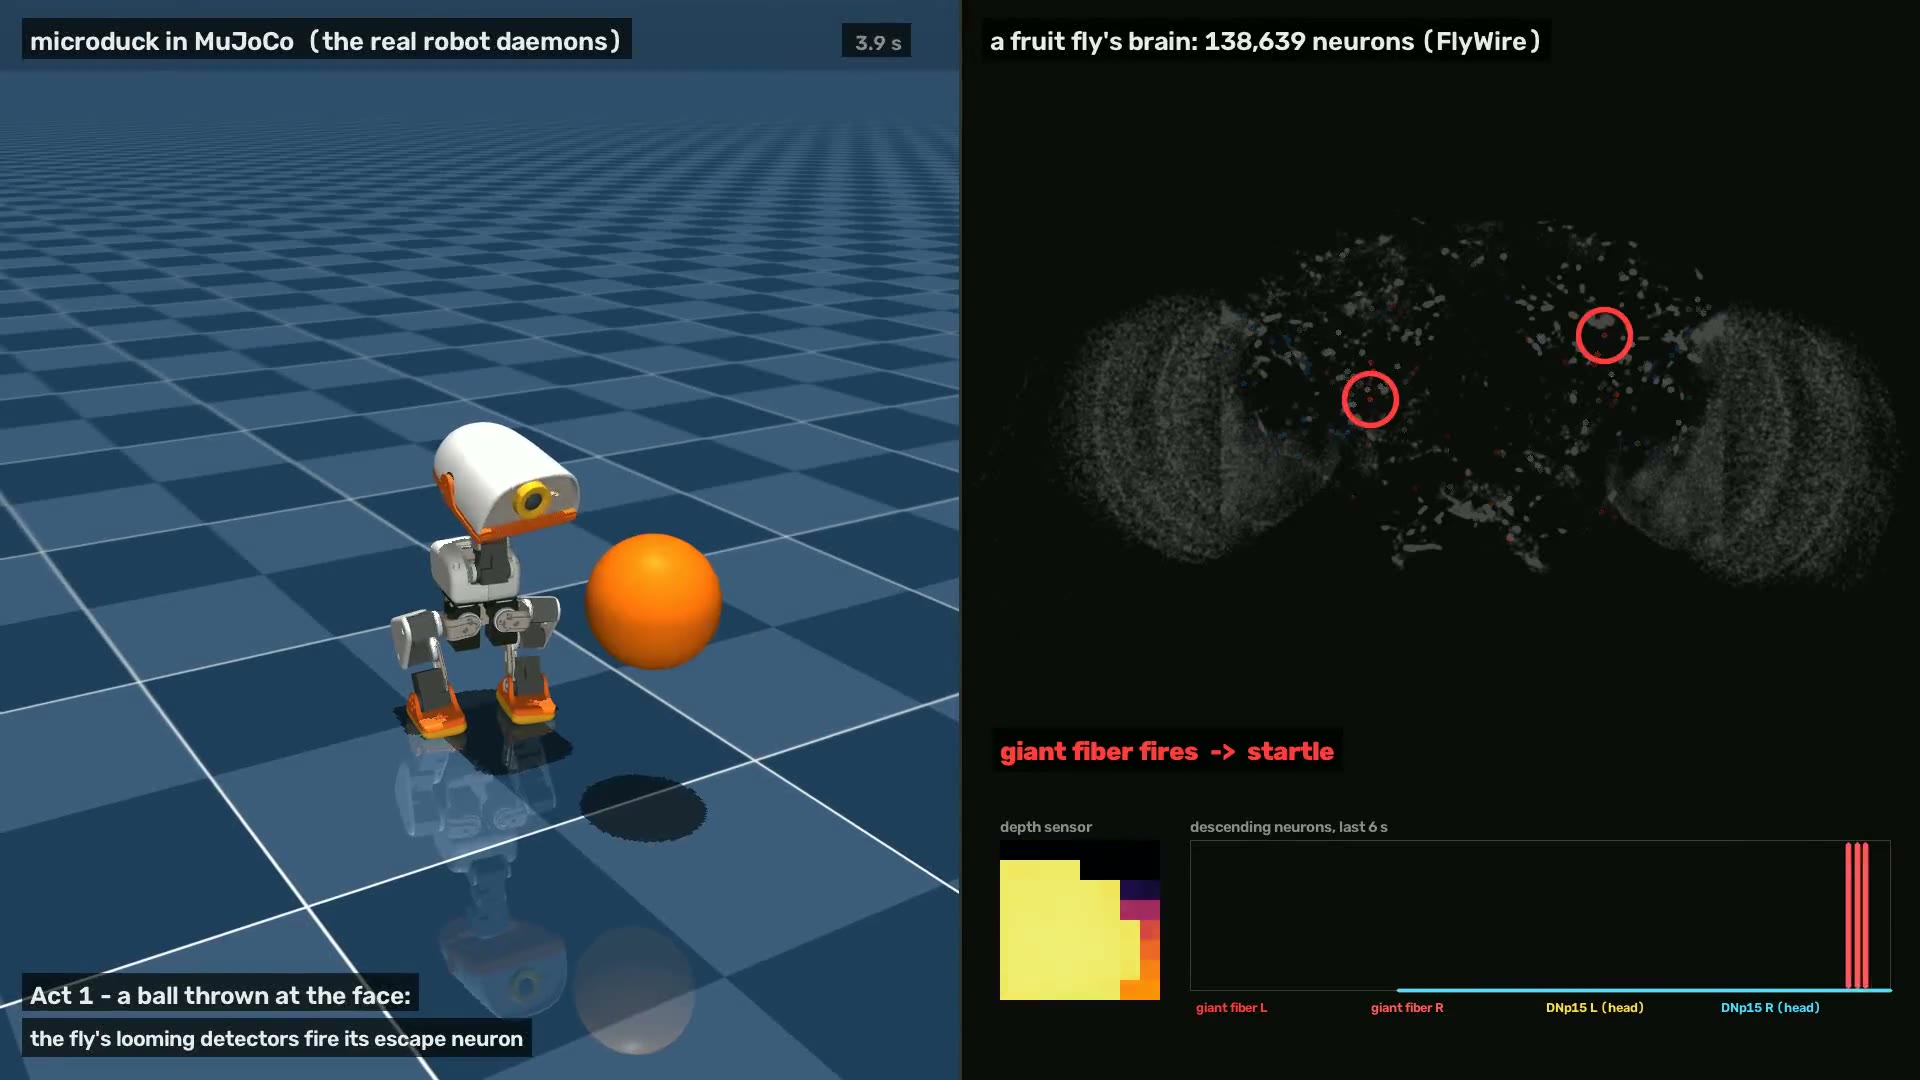
\includegraphics[width=0.49\linewidth]{figures/frame_startle.jpg}\hfill
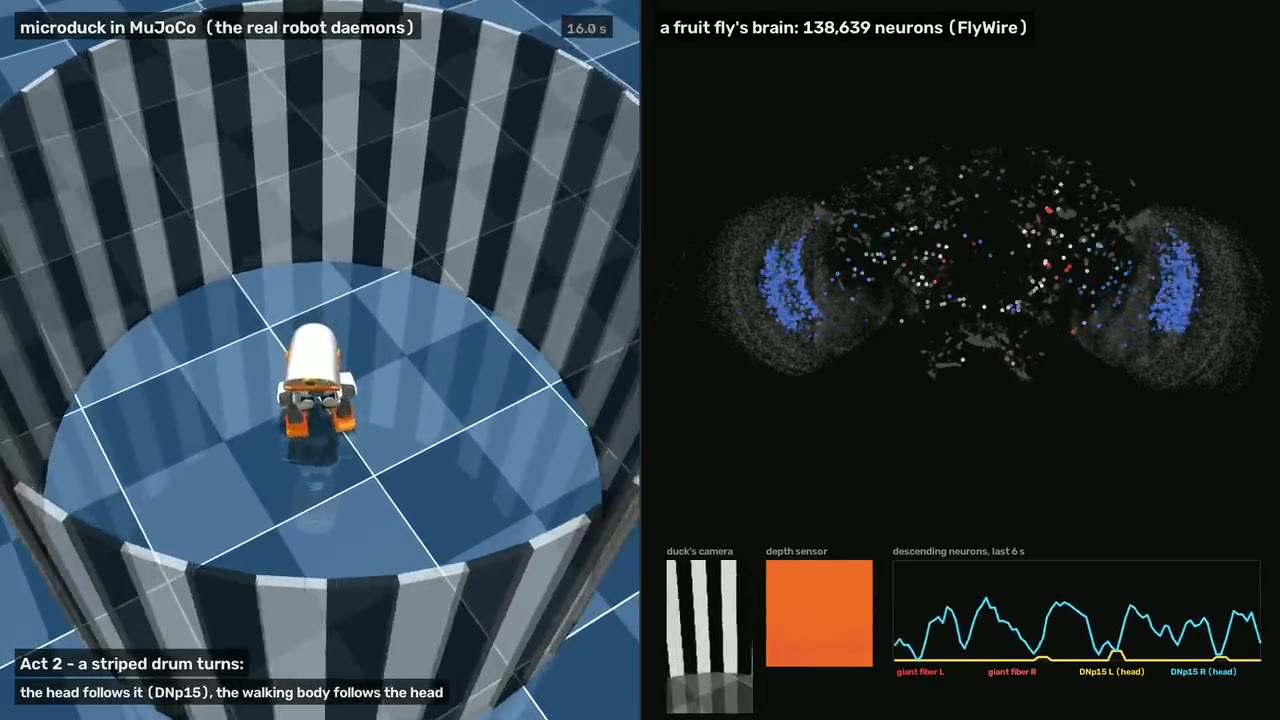
\includegraphics[width=0.49\linewidth]{figures/frame_arena.jpg}
\caption{Frames from the recorded demonstration (\texttt{media/duckophila.mp4}). Left halves: the robot in
MuJoCo, re-rendered from its recorded pose. Right halves: the brain, every neuron at its FlyWire position
seen from the front, lit in its class's colour when it spikes. \textbf{Left:} a ball reaches the robot's
face; both giant fibres are ringed in red as they fire. \textbf{Right:} in the turning drum, T4/T5 neurons
in both optic lobes (blue) and DNp15 respond.}
\label{fig:frames}
\end{figure}

\begin{figure}[t]
\centering
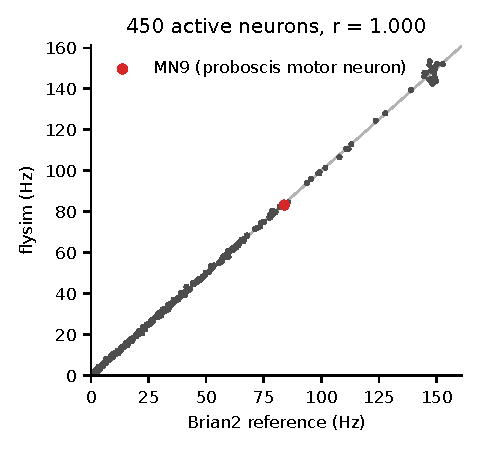
\includegraphics[width=0.36\linewidth]{figures/validation.pdf}
\caption{The stepped simulator against the Brian2 reference: mean firing rates over 30 trials with the
right sugar-sensing neurons at \SI{150}{Hz} (FlyWire 630, as in \cite{shiu2024}).}
\label{fig:validation}
\end{figure}

\subsection{Startle}

Driving LPLC2 and LC4 of one side directly, the giant fibres are silent at rest and fire in a graded way
with drive rate and with the fraction of the population driven, more strongly ipsilaterally; at higher
drive the contralateral DNa01/DNa02 and, weakly, the moonwalker descending neurons (MDN \cite{bidaye2014})
are recruited. On synthetic ToF scenes ray-cast with the sensor's beam geometry and noise (a
\SI{5}{cm} ball approaching from \SI{1.2}{m}, left or right, 40 trials per speed), the giant fibre fired
in 0/40 trials at \SI{0.2}{m/s}, 21/40 at \SI{0.4}{m/s}, 40/40 at each of \SIrange{0.6}{1.5}{m/s}, and
28/40 at \SI{2.0}{m/s}, with a mean latency of \SI{0.54}{s} from onset for approaches $\geq$\SI{1}{m/s}.
Through the full robot stack in the simulator, 20 of 20 balls at \SI{1.5}{m/s} produced a startle
(1.00, 95\% CI [0.84, 1.00]), latency \SI{0.43}{s}, and 0 of 20 hands at \SI{0.2}{m/s}
(Table~\ref{tab:controls}). The speed tuning is largely ours: the approach-speed gate imposes the cut,
and the input null below shows the same cut. Very fast approaches are missed 30\% of the time by the
encoder, and walking towards a wall at \SI{0.3}{m/s} produced a false startle in 6 of 20 trials.

Two failure modes were found and fixed in the interface, not the brain. A standing robot's idle head
motion makes $\sim$45 of 64 depth zones see an approaching and receding floor; without a floor filter 30\%
of quiet frames drove the looming detectors. Near the horizon, a \SIrange{2}{3}{\degree} discrepancy
between the kinematic model and the rendered sensor pose decides whether a grazing return is floor; without
a pose margin, the robot startled 5 times in \SI{25}{s} in an empty room, with it none.

\subsection{Optomotor reflex}

\paragraph{In the connectome.} Driving T4a/T5a of one eye and T4b/T5b of the other---the pattern a yaw
rotation of the world produces---activates the ipsilateral HS cells and contralateral H2 as in the fly,
and flips the left--right activity of DNa02 with the direction of rotation, in the sense of a
syndirectional (following) turn under the interpretation of \cite{rayshubskiy2020}: world turning right,
DNa02 right \SI{28}{Hz} versus left \SI{5}{Hz}; world turning left, left \SI{69}{Hz} versus right
\SI{5}{Hz}. DNa01 does not flip cleanly. The strongest-flipping descending neuron is DNp15 (DNHS1).

\paragraph{Retinotopy is necessary.} With T4/T5 neurons assigned to image regions at random, wide-field
drum motion reached LPLC2 scrambled and fired the giant fibre 7--11 times per run. With column-based
placement, rotation produced no giant-fibre activity in synthetic tests or in the closed loop (one startle
in \SI{29}{s} of drum, from the ToF at start-up).

\paragraph{The camera's field of view limits the readout.} With the column map, a whole-eye yaw rotation
flips both DNa02 and DNp15 (Fig.~\ref{fig:flips}). Restricted to the neurons whose direction falls in the
camera's view, DNp15 still flips strongly (\SI{51}{Hz} left vs.\ \SI{0}{Hz} right; \SI{0} vs.\
\SI{86}{Hz}), but DNa02 does not change sign: right exceeds left in both directions, by \SI{2.7}{Hz} and
\SI{11}{Hz}. Rotation over the frontal \SI{30}{\degree} of the eye at all elevations is sufficient for a
DNa02 flip; the camera's limited elevation range is not. Likewise, no expansion stimulus within the camera
view, up to \SI{400}{\degree/s}, drove LPLC2 appreciably; looming therefore remains the ToF's task.

\paragraph{Closed loop.} With DNp15 driving head yaw, the robot's head follows the drum in both
directions as a triangle wave at about \SI{7}{\degree/s} for a \SI{30}{\degree/s} drum (closed-loop
gain 0.23, 95\% CI [0.21, 0.27], over 12 drum phases: partial compensation) and holds still when the drum is still; higher gains
oscillate, given $\sim$\SI{0.3}{s} of loop latency. With the head-led body coupling, the walking robot
turns with the drum at a mean of $+5$ and \SI{-9}{\degree/s} (peaks $\pm$\SIrange{15}{20}{\degree/s})
against an intrinsic gait drift of \SI{-4.6}{\degree/s}. Without the walking efference copy, three
startles occurred in \SI{200}{s} of walking in the turning drum; with it, none, with unchanged steering.

\begin{figure}[t]
\centering
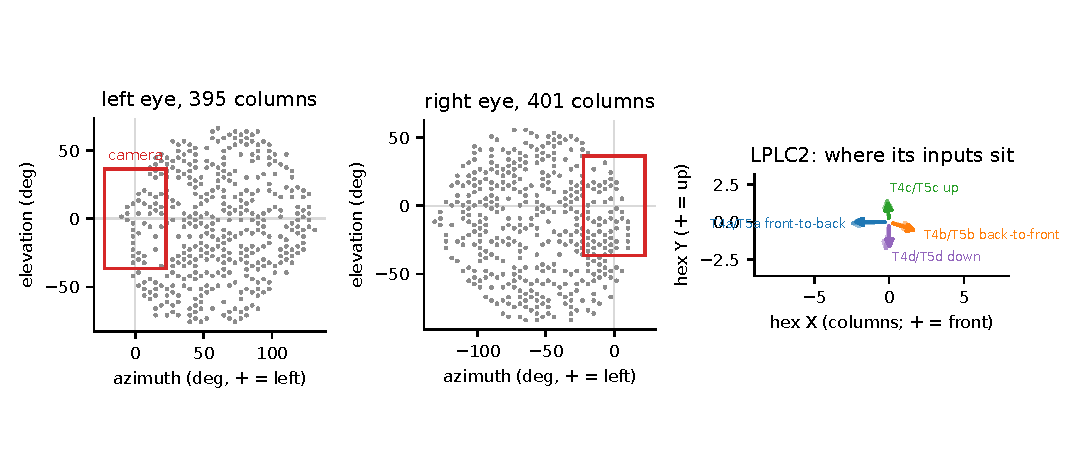
\includegraphics[width=\linewidth]{figures/eyes.pdf}
\caption{Retinotopy from the connectome. \textbf{Left, centre:} viewing directions of the 395 and 401
columns of each eye, from FlyWire's column map with orientation derived from the wiring; red, the camera's
field of view. \textbf{Right:} mean offset of each T4/T5 subtype's input to LPLC2 from the LPLC2 neuron's
input centroid (solid: left eye; faint: right). Front-to-back inputs sit posterior, up inputs dorsal---the
outward-motion arrangement of a looming detector---which fixes the eye's axes.}
\label{fig:eyes}
\end{figure}

\begin{figure}[t]
\centering
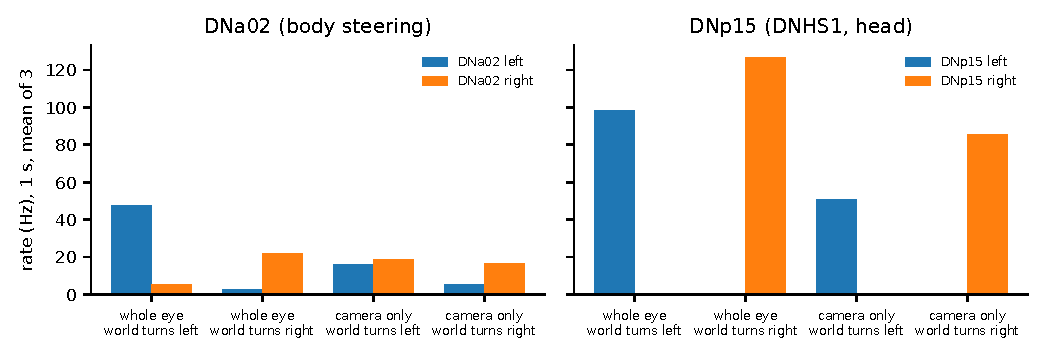
\includegraphics[width=0.9\linewidth]{figures/flips.pdf}
\caption{Steering descending neurons under yaw rotation (\SI{40}{\degree/s}), with every T4/T5 driven
(whole eye) or only those looking into the camera's view. DNp15 flips in both cases; DNa02 only with the
whole eye.}
\label{fig:flips}
\end{figure}

\subsection{Following}

\paragraph{Open loop.} A target \SI{10}{\degree} below the eye's equator makes DNa02 turn toward it,
graded with bearing: left minus right $-5.5$, $-1.8$, $+1.6$, $+5.3$ and \SI{+14.2}{Hz} at $-20$, $-10$,
0, 10 and \SI{20}{\degree} (+ = left; 20 seeds; Fig.~\ref{fig:follow}). Across 383 paired descending
neuron types the left--right difference of nine tracks the bearing ($r > 0.5$); DNa02 ranks third
($r = 0.94$), after DNae002 and DNa16. The rewired brain gives no DNa02 response, and with the same rates
sent to as many random other visual projection neurons the bearing dependence vanishes ($r = 0.05$). Two
properties of the pathway shape the behaviour. It responds to targets below the equator only: the turn
toward a target at $\pm$\SI{10}{\degree} is \SI{0}{Hz} at \SI{+5}{\degree} elevation and above, \SI{2.1}{Hz}
at \SI{-5}{\degree} and \SIrange{3.9}{4.4}{Hz} from \SI{-10}{\degree} down; a target at the camera's height,
which appears above the image centre, is ignored, so the target is on the floor. And it is asymmetric:
the left eye's LC10a receptive fields lie further anterior than the right's (a target dead ahead drives
the left population at \SI{931}{Hz} in total against \SI{782}{Hz}), so DNa02 leans left and a target to
the right gets about a third of the turn of one to the left. Whether this asymmetry is the fly's or our
column-to-angle approximation we cannot tell.

\paragraph{Closed loop.} In 4 of 8 runs the robot kept the target in view throughout, with a heading gain
of 1.00 and a median error of \SI{7.8}{\degree} [7.4, 8.2]. In two of the other four it trailed just
outside the camera's half-width (at most \SI{29}{\degree}) from the first reversal on and kept turning
with the target (gain 1.00 and 0.94); in two it fell further behind after a reversal and lost the target
for part of the run (gain 0.56 and 0.69). Over all eight runs the mean heading gain was 0.90 [0.78, 1.00]. The rewired brain never followed (0 of 8, 95\% CI [0.00, 0.32];
gain $-0.01$). No run of either brain produced a startle.

\paragraph{A person's feet.} Open loop, synthetic motion at \SI{15}{\degree} to the left through the
pooling (with a \SI{5}{\degree} reference disc) turned DNa02 by \SI{+10.7}{Hz} for a ball-sized patch and
\SI{+12.3}{Hz} for two feet low in the view, but by \SI{+0.3}{Hz} for the same feet with whole legs above
them to \SI{+30}{\degree}: too much of the small-object pathway driven at once no longer steers, which is
why only each blob's lowest part drives it. On the stepping legs in closed loop, DNa02 alone did not
steer: it fires a few spikes a second, and its left--right difference (\SI{+4.8}{Hz} with the person on
the left, \SI{+2.3}{Hz} ahead, \SI{+0.1}{Hz} on the right) drowned in their noise. Of 383 paired DN types,
DNae002 and DNa16 follow a target's bearing more steeply than DNa02 (9.5 and 6.4 against 4.6\,Hz per
\SI{10}{\degree}; DNg97 $-3.5$), and their combined difference changed sign between the sides
(\SI{+36}{Hz} left, \SI{-12}{Hz} right) but leant left, \SI{+13.5}{Hz} with the person dead ahead---in
proportion to the LC10a drive, and absent in the rewired brain, whose readout neurons do not respond.
Each further rule answered a measured failure: walking toward the person made the floor flow through the
lower field and the intact brain followed its own flow round in circles; a turn the DNs kept up after a
fast turn of the robot's own carried it into a spin; and the legs, \SI{0.6}{m} away, loomed on the depth
sensor and fired the giant fibre $\sim$8 times a run, each flinch breaking the following. Walking after
the person needed more: a shift does not take the gait's rocking off the image (offline, in an empty room,
5--7\% of it still moved; a field predicted from the robot's state, 10\%; the image's homography, 0.1--0.3\%);
feet more than $\sim$\SI{0.8}{m} away sat above the camera's centre and so, mapped as the camera, above
the fly's equator; and by moving area distant feet drove LC10a too little (open loop, two feet
\SI{1.5}{m} away gave $\pm$\SI{3}{Hz}; as point targets, $-40$ and \SI{+47}{Hz}). With all of it (Methods),
over 8 runs each: round the robot the intact brain kept a heading gain of 0.67 [0.32, 0.94] (median error
\SI{32}{\degree} [15, 56], the person in view 51\%), the rewired brain 0.02 (\SI{40}{\degree}, 35\%---the
share a robot that does not turn keeps in view); the glowing ball, 0.90. Walking away, the intact robot
walked \SI{1.28}{m} [0.61, 1.98] after the person against \SI{0.41}{m}, at a median distance of \SI{1.78}{m}
against \SI{2.33}{m}; it kept up in 3 of 8 runs (the best \SI{2.9}{m} walked, \SI{7}{\degree} median error,
in view 77\%), and the rewired robot in none; in the others it lost the person at a curve. On the four
phone clips, open loop, the encoder and brain turned toward the walking person 90\% of the time they
turned and not at all in the empty room standing, but 39\% of the time in the empty room while the phone
turned through chair legs a hand's breadth away: their parallax is no single homography, and a point
target counts in full where moving area did not (the area pooling, before the walking, turned there 1\%). Tracking each object, so that only one found again
at its place for 12 frames counts in full, cut that to 7\% on the clip but in the simulator halved the
gain round the robot and stopped it walking after the person; it is not used. Three clips filmed
afterwards, on which nothing was tuned: in another room, in daylight, it turned toward the walking
person 94\% of the time it turned; with the phone held low behind walking feet, close up, 66\%; a
rolling black ball it hardly registered (large, dark and untextured, only its edges and shadow moved). Integrate-and-fire saccades on
the same readout \cite{mongeau2017} also followed but overshot; a single equator for both eyes (HSE's
input centroid, one cell per eye, puts them $\sim$\SI{10}{\degree} apart on an otherwise identical column
grid) did not remove the lean.

\begin{figure}[t]
\centering
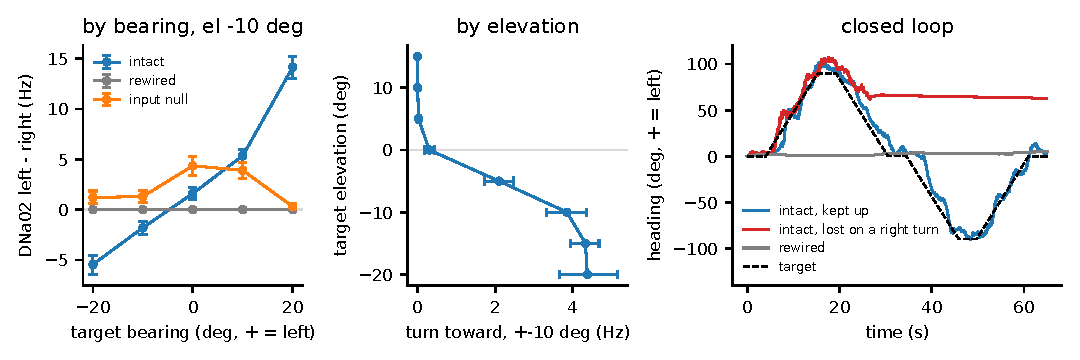
\includegraphics[width=\linewidth]{figures/follow.pdf}
\caption{Following. \textbf{Left:} DNa02 left minus right against the target's bearing, open loop (mean,
95\% CI, 20 seeds), for the intact brain, the rewired brain, and the input null. \textbf{Centre:} the turn
toward a target \SI{10}{\degree} out, against its elevation. \textbf{Right:} closed loop, the robot's
heading against the target's for a run that kept up, one that fell behind after a reversal, and the
rewired brain.}
\label{fig:follow}
\end{figure}

\subsection{The mushroom body, and learning}

\paragraph{No code of its own.} Kenyon cells take visual input mainly in KCg-d (30\% of their input
synapses, from aMe12 and medulla/lobula projection neurons; KCab-p 3\%, others $<$1\%). Nothing the
camera can drive reaches them: rotation on the camera's T4/T5, the follow target on LC10a, a
\SI{10}{\degree} patch on every columnar neuron, and all 45{,}528 columnar neurons at \SI{30}{Hz} each
fire none of the 31 visual projection neurons that feed Kenyon cells, which take only 3\% of their
input from column-mapped neurons. More fundamentally, the model's Kenyon cells do not code their
input. Four odours (one olfactory receptor neuron type each) and taste either reach no Kenyon cell or
the same $\sim$3{,}370 of 5{,}177 (Jaccard overlap 0.99--1.00), with the whole brain at
$\sim$\num{470000} spikes/s; a fly uses a sparse, odour-specific 5--10\%. Removing the Kenyon cells'
synapses onto each other (38\% of their output weight) leaves it so (overlap $\geq 0.98$). The runaway
begins in the antennal lobe, whose local and projection neurons fire just before the Kenyon cells
do; with the antennal lobe silenced, a random 15\% of Kenyon cells at \SI{20}{Hz} never ran away
(0 of 10, intact 3 of 10). In this model the dopamine neurons, like every other synapse whose
transmitter is not GABA or glutamate, are excitatory.

\paragraph{Open loop.} With the additions above, pairing cue A four times with petting raised its
value over that of an unpaired cue B by \SI{3.35}{Hz} [2.83, 3.82] (10 seeds). The same cue and the
same petting on separate trials ($-0.39$ [$-0.94$, 0.14]) and no petting ($-0.12$ [$-0.70$, 0.45])
did not; in the rewired brain nothing changed (0.00). With valence read off the MBONs' transmitters
instead (glutamate avoidance, acetylcholine and GABA approach \cite{aso2014b}), petting made the
paired cue \emph{less} attractive, almost entirely through the GABAergic MBON09 in a PAM compartment.

\paragraph{Closed loop.} Six runs per brain, the petted target alternating between ball and bar.
Naive, the robot followed neither (0 of 6 each). After four 3-s pettings with one target in view
and four presentations of the other, the petted target's value had risen by 3.8--4.2\,Hz and the
other's by 0.3--0.6\,Hz in all six runs; the robot then walked after the petted target in 5 of 6 runs
(net \SI{1.03}{m} [0.70, 1.26] in \SI{30}{s}; heading gain 0.76 [0.41, 0.96]; ball and bar both) and
after the other in none. The failure learned but lost the target while following. The rewired brain learned and followed nothing.

\subsection{Controls}

To ask what the connectome contributes, we repeated each experiment with brains that are wrong in one
respect (Table~\ref{tab:controls}): a \emph{rewired} connectome, in which every connection keeps its
presynaptic neuron and weight but receives a target from a random permutation of all targets (so every
neuron keeps its in- and out-degree); a \emph{sign-flipped} connectome; an \emph{input null}, the intact
brain with the looming encoder's output sent to as many randomly chosen other visual projection neurons of
the same side; and a \emph{readout null}, every descending neuron type with exactly one neuron per side
scored for following rotation.

The rewired and sign-flipped brains remain active---\num{55000} spikes per second under visual drive,
against \num{66000} intact---but activity no longer reaches the descending neurons: no startle in any of
280 open-loop or 20 closed-loop trials, no DNp15 or DNa02 response, and a closed-loop head gain of 0.00.
DNp15's following is specific: of 383 paired descending neuron types, 13 follow a rotation within the
camera's view (95\% CIs excluding zero in both directions) and DNp15 follows most strongly (rank 1, as also
over the whole eye). The escape response is less specific than the demonstrations suggest: the input null
still fired the giant fibre in about half of fast approaches (0.50 [0.35, 0.65] at \SIrange{0.6}{1.5}{m/s},
against 1.00 for LPLC2/LC4), so in this model the giant fibre can be reached from visual input in general,
and LPLC2/LC4 make it reliable. Laterality is weak: the giant fibre ipsilateral to the ball carried 58\% of
giant-fibre spikes (95\% CI [56, 59]) in open loop and 57\% [45, 66] in closed loop, close to the input
null's 54\% [52, 56].

\begin{table}[t]
\centering\small
\caption{Controls. Open loop: 20 seeds per condition (40 trials per speed across both sides); closed loop:
20 throws, 8 following and 6 learning runs, through the full robot stack. 95\% Wilson (proportions) or bootstrap (means) intervals.}
\label{tab:controls}
\begin{tabular}{lcccc}
\toprule
 & intact & rewired & sign-flipped & input null \\
\midrule
Startle, \SIrange{0.6}{1.5}{m/s}, open loop & 1.00 [0.91, 1.00] & 0.00 & 0.00 & 0.50 [0.35, 0.65] \\
Startle, \SI{0.2}{m/s}, open loop & 0.00 [0.00, 0.09] & 0.00 & 0.00 & 0.00 \\
Startle, \SI{1.5}{m/s}, closed loop & 1.00 [0.84, 1.00] & 0.00 [0.00, 0.16] & & \\
Startle, \SI{0.2}{m/s}, closed loop & 0.00 [0.00, 0.16] & 0.00 [0.00, 0.16] & & \\
Ipsilateral GF spike share & 0.58 [0.56, 0.59] & -- & -- & 0.54 [0.52, 0.56] \\
False startle, walking at a wall \SI{0.3}{m/s} & 6/20 & 0/20 & 0/20 & 2/20 \\
Head optomotor gain, closed loop & 0.23 [0.21, 0.27] & 0.00 & & \\
DNp15 follows rotation (camera view) & yes, rank 1/383 & no & no & \\
DNa02 follows rotation & whole eye only & no & no & \\
DNa02 tracks target bearing, open loop & $r = 0.94$, rank 3/383 & $r = 0.00$ & & $r = 0.05$ \\
Following, runs kept up, closed loop & 4/8 [0.22, 0.78] & 0/8 [0.00, 0.32] & & \\
Following feet round the robot, heading gain & 0.67 [0.32, 0.94] & 0.02 & & \\
Walking after feet: runs kept up, metres walked & 3/8, \SI{1.28}{m} & 0/8, \SI{0.41}{m} & & \\
Learning index, open loop (Hz) & +3.35 [2.83, 3.82] & 0.00 & & \\
Walks after petted / other target & 5/6 / 0/6 & 0/6 / 0/6 & & \\
\bottomrule
\end{tabular}
\end{table}

\section{Discussion}

The connectome, unmodified and untrained, produced three recognisable fly behaviours when its sensory
neurons were driven by a robot's sensors: an escape decision to fast approaching objects, a following
optomotor response, and turning toward a small object. None was wired in, and all disappear when the same
neurons and weights are rewired. Their specificity differs: the optomotor readout singles out DNp15 among hundreds of candidates,
whereas the escape decision is made more reliable, but not made possible, by the looming detectors, and
carries little information about the side of the threat. An earlier, demonstration-based version of these
results described the escape as lateralised; the controls do not support that. What was wired in is listed in
Table~\ref{tab:boundary}, and most of the effort went there: the biological plausibility of the input
decided whether the connectome's computation could be expressed at all. Scrambled retinotopy did not just
add noise, it produced false escape decisions, because LPLC2's selectivity is a property of where its
inputs sit. The robot's own movement dominated its visual input, as it does for animals, and needed an
efference copy before the fly's motion pathway could be used while walking \cite{kim2015}.

The clearest limitation is sensory. A single forward camera covers a small part of a fly's visual field,
and the canonical steering neuron DNa02 \cite{rayshubskiy2020} did not respond to rotation within it. The
head-coupled neuron DNp15 did, so we steer the head with the fly's output and the body with a coupling rule
of ours. Whether a wider camera, or several, recover DNa02-based steering is a direct experimental question
the setup can answer. For a small target DNa02 does respond within the camera's view, so following is
steered by the fly's own steering neuron; but its losses---a target that leaves the \SI{45}{\degree} view
is not found again---are again the camera's, against a fly's nearly panoramic eyes.

Other limitations are those of the model and the platform. The LIF model of \cite{shiu2024} uses one
synaptic weight for all connections, has no gap junctions (the giant fibre's electrical synapses are
absent), no plasticity and no neuromodulation, and treats neurotransmitter predictions as signs. T4 and T5
are driven alike, without an ON/OFF split. The robot is simulated; its gait reaches 40\% of commanded speed
and the camera/state timing measured in simulation will differ on hardware. Our gains and gates are
engineering choices, stated as such. With the self-lit target, LC10a's preference for moving over
stationary objects is not modelled; with the motion encoder only what moves drives it.
We make no claim that the robot behaves like a fly beyond the three behaviours measured.

Following a person shows where the boundary moves when the input is real. The pathway is the
fly's---two feet low in the view steer DNa02 as a target does, the whole legs do not, and nothing
follows when the wiring is rewired---but steering from it took more of ours than following a glowing
target did: a readout over four DN pairs instead of one, a correction for a lean that appears in our
receptive-field map, the room's homography, and rules for a body that moves its own camera (keeping its distance, a heading
memory, suppression during its own fast turns, a search the brain's way, no flinch at what it pursues).
Several have counterparts in flies, population readout of descending neurons, saccadic suppression, a
compass in the central complex, a memory for a vanished object,
but here they are rules, not circuits. The lean is likely ours as well: the two eyes' maps differ by
$\sim$\SI{10}{\degree} in elevation where their column grids do not, which a better placement of each eye's
equator than one cell's input centroid should settle.

Learning is different in kind. The model's mushroom body does not code its input, so the cue codes,
the plasticity, the valence assignment and a lesion are ours, and what the connectome contributes is
narrower: the Kenyon cell $\rightarrow$ MBON wiring and its compartments, which carry a cue-specific,
pairing-specific change through to behaviour and fail to when rewired. Why the reference model's
antennal lobe runs away---one shared synaptic weight, no graded inhibition, excitatory
neuromodulators---is a question for the model, and a prerequisite for using it to study learning.

The natural next step is the physical robot. The path to it is in place: the brain on a laptop,
reaching the robot over the WebRTC session it publishes, with frames dated on the robot's clock
(Methods); what remains is to measure the real camera's delay, as was done in simulation. Related efforts embody
connectome-constrained or neuromechanical fly models in simulated bodies \cite{lobato2022,vaxenburg2025};
here the body is a different animal's, and the interesting part is the translation between them.

\section*{Reproducibility}

Everything above is a script in \url{https://github.com/first-it-consulting/duckophila}:
\texttt{experiments/} (each figure and number), \texttt{paper/figures.py} (every figure, from data),
\texttt{demo.sh --video} (the recorded demonstration). The FlyWire data are fetched under their own terms.
Hardware: Apple M5 Max, macOS; brain on one core.

\section*{Acknowledgements}

The connectome and annotations are the work of the FlyWire consortium; the brain model is that of Shiu et
al.; the robot, its software and its simulator are Pollen Robotics'. The FlyWire annotations used are
version $\geq$3.2, for which the annotation authors also ask to cite Berg et al.\ (2026) and Tastekin et
al.\ (2026). The implementation, experiments and this report were developed with substantial assistance
from an AI coding assistant (Anthropic's Claude), directed and reviewed by the author.

\begin{thebibliography}{99}\small
\bibitem{dorkenwald2024} S.~Dorkenwald et al. Neuronal wiring diagram of an adult brain. \emph{Nature} 634, 124--138 (2024).
\bibitem{schlegel2024} P.~Schlegel et al. Whole-brain annotation and multi-connectome cell typing of \emph{Drosophila}. \emph{Nature} 634, 139--152 (2024).
\bibitem{matsliah2024} A.~Matsliah et al. Neuronal parts list and wiring diagram for a visual system. \emph{Nature} 634, 166--180 (2024).
\bibitem{shiu2024} P.~K.~Shiu et al. A \emph{Drosophila} computational brain model reveals sensorimotor processing. \emph{Nature} 634, 210--219 (2024).
\bibitem{stimberg2019} M.~Stimberg, R.~Brette, D.~F.~M.~Goodman. Brian 2, an intuitive and efficient neural simulator. \emph{eLife} 8, e47314 (2019).
\bibitem{todorov2012} E.~Todorov, T.~Erez, Y.~Tassa. MuJoCo: a physics engine for model-based control. \emph{IROS} (2012).
\bibitem{maisak2013} M.~S.~Maisak et al. A directional tuning map of \emph{Drosophila} elementary motion detectors. \emph{Nature} 500, 212--216 (2013).
\bibitem{klapoetke2017} N.~C.~Klapoetke et al. Ultra-selective looming detection from radial motion opponency. \emph{Nature} 551, 237--241 (2017).
\bibitem{vonreyn2017} C.~R.~von Reyn et al. Feature integration drives probabilistic behavior in the \emph{Drosophila} escape response. \emph{Neuron} 94, 1190--1204 (2017).
\bibitem{ache2019} J.~M.~Ache et al. Neural basis for looming size and velocity encoding in the \emph{Drosophila} giant fiber escape pathway. \emph{Curr.\ Biol.} 29, 1073--1081 (2019).
\bibitem{namiki2018} S.~Namiki, M.~H.~Dickinson, A.~M.~Wong, W.~Korff, G.~M.~Card. The functional organization of descending sensory-motor pathways in \emph{Drosophila}. \emph{eLife} 7, e34272 (2018).
\bibitem{rayshubskiy2020} A.~Rayshubskiy et al. Neural circuit mechanisms for steering control in walking \emph{Drosophila}. \emph{bioRxiv} (2020).
\bibitem{bidaye2014} S.~S.~Bidaye, C.~Machacek, Y.~Wu, B.~J.~Dickson. Neuronal control of \emph{Drosophila} walking direction. \emph{Science} 344, 97--101 (2014).
\bibitem{kim2015} A.~J.~Kim, J.~K.~Fitzgerald, G.~Maimon. Cellular evidence for efference copy in \emph{Drosophila} visuomotor processing. \emph{Nat.\ Neurosci.} 18, 1247--1255 (2015).
\bibitem{farneback2003} G.~Farneb\"ack. Two-frame motion estimation based on polynomial expansion. \emph{Scandinavian Conference on Image Analysis} (2003).
\bibitem{lobato2022} V.~Lobato-Rios et al. NeuroMechFly, a neuromechanical model of adult \emph{Drosophila melanogaster}. \emph{Nat.\ Methods} 19, 620--627 (2022).
\bibitem{vaxenburg2025} R.~Vaxenburg et al. Whole-body physics simulation of fruit fly locomotion. \emph{Nature} (2025).
\bibitem{ribeiro2018} I.~M.~A.~Ribeiro et al. Visual projection neurons mediating directed courtship in \emph{Drosophila}. \emph{Cell} 174, 607--621 (2018).
\bibitem{hindmarshsten2021} T.~Hindmarsh Sten, R.~Li, A.~Otopalik, V.~Ruta. Sexual arousal gates visual processing during \emph{Drosophila} courtship. \emph{Nature} 595, 549--553 (2021).
\bibitem{caron2013} S.~J.~C.~Caron, V.~Ruta, L.~F.~Abbott, R.~Axel. Random convergence of olfactory inputs in the \emph{Drosophila} mushroom body. \emph{Nature} 497, 113--117 (2013).
\bibitem{hige2015} T.~Hige, Y.~Aso, M.~N.~Modi, G.~M.~Rubin, G.~C.~Turner. Heterosynaptic plasticity underlies aversive olfactory learning in \emph{Drosophila}. \emph{Neuron} 88, 985--998 (2015).
\bibitem{cohn2015} R.~Cohn, I.~Morantte, V.~Ruta. Coordinated and compartmentalized neuromodulation shapes sensory processing in \emph{Drosophila}. \emph{Cell} 163, 1742--1755 (2015).
\bibitem{aso2014b} Y.~Aso et al. Mushroom body output neurons encode valence and guide memory-based action selection in \emph{Drosophila}. \emph{eLife} 3, e04580 (2014).
\bibitem{owald2015} D.~Owald, S.~Waddell. Olfactory learning skews mushroom body output pathways to steer behavioral choice in \emph{Drosophila}. \emph{Curr.\ Opin.\ Neurobiol.} 35, 178--184 (2015).
\bibitem{mongeau2017} J.-M.~Mongeau and M.~A.~Frye. \emph{Drosophila} spatiotemporally integrates visual signals to control saccades. \emph{Curr. Biol.} 27, 2901--2914 (2017).
\bibitem{neuser2008} K.~Neuser, T.~Triphan, M.~Mronz, B.~Poeck and R.~Strauss. Analysis of a spatial orientation memory in \emph{Drosophila}. \emph{Nature} 453, 1244--1247 (2008).
\end{thebibliography}

\end{document}
